%%% template.tex
%%%
%%% This LaTeX source document can be used as the basis for your technical
%%% paper or abstract. Regardless of the length of your document, the commands
%%% are all the same.
%%% 
%%% The "\documentclass" command is the first command in your file. If you want to 
%%% prepare a version of your article with line numbers - a "review" version - 
%%% include the "review" parameter:
%%%    \documentclass[review]{acmsiggraph}
%%%

\documentclass{acmsiggraph}
\usepackage{xcolor,colortbl}
\usepackage{multirow}
\usepackage[export]{adjustbox}
\usepackage{enumitem}

%%% Title of your article or abstract.

\title{Fourier Analysis of Numerical Integration in Monte Carlo Rendering:  \\Theory and Practice}

\author{
Kartic Subr  \thanks{e-mail:k.subr@hw.ac.uk}\\Heriot Watt University 
\and Wojciech Jarosz  \thanks{e-mail:wojciech.k.jarosz@dartmouth.edu}\\Dartmouth College
\and Gurprit Singh  \thanks{e-mail:gurprit.singh@dartmouth.edu}\\Dartmouth College
}
\pdfauthor{Kartic Subr}

%%% Used by the ``review'' variation; the online ID will be printed on 
%%% every page of the content.

\TOGonlineid{45678}

% User-generated keywords.

\keywords{Fourier analysis, Monte Carlo sampling, numerical integration}

% With the "\setcopyright" command the appropriate rights management text will be added
% to your document.

%\setcopyright{none}
%\setcopyright{acmcopyright}
%\setcopyright{acmlicensed}
\setcopyright{rightsretained}
%\setcopyright{usgov}
%\setcopyright{usgovmixed}
%\setcopyright{cagov}
%\setcopyright{cagovmixed}
%\setcopyright{rightsretained}

% The year of publication in the "\copyrightyear" command.

\copyrightyear{2016}

%%% Conference information, from the completed rights management form.
%%% The "\conferenceinfo" command has two parameters: 
%%%    - conference name
%%%    - conference date and location
%%% The "\isbn" field includes the year and month after the article ISBN.

\conferenceinfo{SIGGRAPH 2016 Posters}{July 24-28, 2016, Anaheim, CA} 
\isbn{978-1-4503-ABCD-E/16/07} 
\doi{http://doi.acm.org/10.1145/9999997.9999999}

\begin{document}

%%% This is the ``teaser'' command, which puts an figure, centered, below 
%%% the title and author information, and above the body of the content.

 \teaser{
   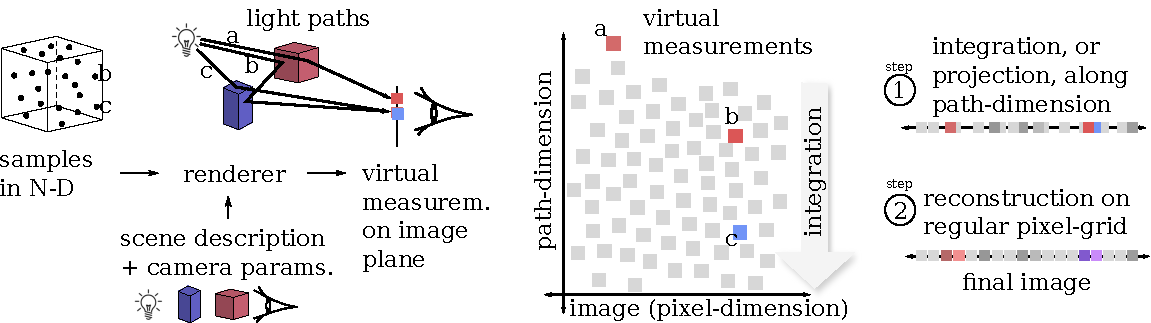
\includegraphics[height=1.6in]{../CourseNotes/Pictures/RenderHL.pdf}
   \caption{}
   \label{fig:renderhl}
 }

\maketitle

\begin{abstract}

Since being introduced to graphics in the 1980s, Monte Carlo sampling has become the cornerstone of most modern algorithms that are used to generate high-quality, photorealistic imagery. Originally introduced to combat the effect of aliasing when estimating values at pixels, it has attained popularity as a general tool for solving complex, multi-dimensional integration problems in rendering. In this context, MC integration involves \textit{sampling} a function at various stochastically placed points and averaging the sampled values to approximate an integral, e.g. the radiance through a pixel integrated across the multi-dimensional space of possible light transport paths. Unfortunately, such estimation is error-prone and the visual manifestation of this error depends critically on the properties of the integrand, placement of the stochastic sample points used, and the type of problem (integration vs.\ reconstruction) that is being solved with these samples.

Fourier analysis, along with the Nyquist theorem, have long been used in graphics to motivate more intelligent sampling strategies which try to minimize errors due to noise and aliasing in the \textit{pixel reconstruction problem}. Only more recently, however, has the community started to apply these same Fourier tools to analyze error in the Monte Carlo \textit{integration problem}. Loosely speaking, in the context of rendering a 2D image, these two problems are concerned with errors introduced across pixels (reconstruction) vs.\ the errors introduced within any individual pixel (integration). In this course, we focus on the latter, and survey the recent developments and insights that Fourier analyses have provided about the magnitude and convergence rate of Monte Carlo integration error. We provide a historical perspective of Monte Carlo in graphics, review the necessary mathematical background, summarize the most recent developments, discuss the practical implications of these analyzes on the design of Monte Carlo rendering algorithms, and identify important remaining research problems that can propel the field forward.

\end{abstract}

%
% The code below should be generated by the tool at
% http://dl.acm.org/ccs.cfm
% Please copy and paste the code instead of the example below. 
%
\begin{CCSXML}
<ccs2012>
<concept>
<concept_id>10010147.10010371.10010372</concept_id>
<concept_desc>Computing methodologies~Rendering</concept_desc>
<concept_significance>500</concept_significance>
</concept>
<concept>
<concept_id>10010147.10010371.10010372.10010374</concept_id>
<concept_desc>Computing methodologies~Ray tracing</concept_desc>
<concept_significance>100</concept_significance>
</concept>
</ccs2012>
\end{CCSXML}

\ccsdesc[500]{Computing methodologies~Rendering}
% \ccsdesc[100]{Computing methodologies~Ray tracing}
%
% End generated code
%

% The next three commands are required, and insert the user-generated keywords, 
% The CCS concepts list, and the rights management text.
% Please make sure there is a blank line between each of these three commands.

\keywordlist

% \conceptlist

\printcopyright

\section{Estimation errors due to sampling patterns}
Modern algorithms that are used to generate high-quality photorealistic pictures proceed by simulating the flow of radiant spatio-directional light energy (radiance) within environments. Given the geometric and material specifications of the objects in any scene, most \textit{renderers} output simulated images as seen through a virtual camera whose parameters are pre-specified (Fig.~\ref{fig:renderhl}.i). Such renderers essentially perform two important steps (Fig.~\ref{fig:renderhl}.iii): 1) they \textit{estimate} the radiance arriving at various points on the virtual sensor by integrating the simulated measurement contributions over paths; 2) they \textit{reconstruct} the output image by resampling the estimated values on a regular grid of pixel-centers that lie on the virtual sensor. This course is dedicated to understanding estimation errors.

The typical approach for estimation proceeds by implicitly mapping high-dimensional random samples to \textit{important} light paths in the scene (Fig.~\ref{fig:renderhl}.i), followed by a carefully-weighted deposition of the radiance contributed by each path as it impinges on the image plane. The efficiency of \textit {Monte Carlo renderers} can be quantified by how rapidly the image plane is populated with important estimates of radiance. The quality of the resulting estimation crucially depends on the statistical properties of the \textit {sampling pattern}, or the sum of impulses in the high-dimensional input space, which is used to generate the paths. To be practically useful, a renderer must be both efficient as well as able to generate ``high-quality'' estimation. The quality of estimation of global illumination, is plagued by error from many sources~\cite{arvo1994framework}. 


% Beyond these objectives, we envision that this course will stimulate the development of new sampling algorithms.~e.g.~Knowledge of the Fourier properties of the underlying integrand (radiance function) via rapid measurements of local variation may be exploited to design sampling patterns for the specific scene rather than merely using this information to adapt sampling density~\cite{Cov5D}.

During the process of estimation, multiple (vastly different) paths may co-incide on any given pixel. At one such pixel, imagine storing an array of \textit{all} the radiance values contributed by the paths arriving there. The histogram of this array is representative of the distribution of radiance at that pixel. The difference between the expected value of this distribution (or the average of the values in the array) and the true radiance at the pixel, \textit{bias} of the estimator, quantifies the accuracy of the simulation.  The second central moment of the distribution (or the \textit{variance} of the values in the array) quantifies the precision of the estimator. The behaviour of bias and variance at a pixel as the number of paths contributing radiance to that pixel increases is called the \textit{convergence rate}. 

In practice, errors in estimation appear in the image as coherent structured artifacts (e.g.~banding), low-frequency smears and high-frequency noise. The first two are attributed to bias, while the third is attributed to variance. Although each pixel in an image is assigned a single, averaged estimate, poor precision leads to disagreement between estimates of neighboring pixels. If these neighboring pixels lie on what should be a smooth part of the image, the disagreement manifests as noise.

\section{Need for analysis of error in rendering}

While some estimators exhibit higher error than others for a budget of (say) 10 samples per pixel, their better convergence rate could lead to dramatically superior rendering at a higher computational budget of (say) 1000 samples per pixel.~i.e.~the estimator of choice for a scene may also depend on the computational budget (interactive vs offline rendering). Recent works have derived mean-squared error~\cite{durand2011frequency,Ramamoorthi:2012}, variance~\cite{Subr:2013:FAS,subr14error} and convergence rates~\cite{Pilleboue:2015:VAM} as functions of the Fourier statistics of typical sampling patterns that are used in Monte Carlo rendering. A thorough understanding of error will allow informed choices potentially leading to the use of the ``best available'' sampling strategy for a given scene and computational budget. 

\section{Course scope and relevance at SIGGRAPH}
Modern Monte Carlo renderers are large and sophisticated systems with numerical integration at their very crux. This course will focus on understanding estimation errors, in the Fourier domain, that arise during numerical integration of radiance values. The focus of this course is complementary to previous rendering courses. This novel course will explain the impact of sampling patterns with desirable Fourier characteristics on estimation error by surveying a number of recent works.

Fourier analysis is also extensively used in the design of computational displays and cameras. Our focus on numerical integration is fundamentally different than those applications, where integration happens physically (implicitly) by propagation of real light energy  (e.g.~blurring of images due to a wide aperture). There have been conspicuously few courses on the application of Fourier analysis at SIGGRAPH and we believe that the sections containing generalized treatment of the problem will provide valuable insights into applications other than rendering. Finally, we envision this course to stimulate the development of new sampling algorithms when partial information is available about the integrand~\cite{Cov5D}.

\section{Course overview and objectives}
This course schedule is shown in table~\ref{tab:ovw}. The content for the course will be a combination of intuition and insights (presentation slides), formal mathematical content (course material) as well as visualization and live demonstration (with source code). We attach a sample of the course notes.
At the end of this course, attendees will 
\begin{itemize}[noitemsep,topsep=-1em,leftmargin=*]
\item understand the impact of sampling patterns on MC integration
\item be aware of the state of the art in sampling for MC rendering
\item understand the main sources of error in MC rendering 
\item internalize the difference between error and convergence rate
\item appreciate the Fourier perspective of MC integration
\item be able to identify different spectral signatures of sampling patterns that may indicate potential for high error
\item develop an intuition for sampling patterns that lead to high error
\item be equipped with mathematical tools as well as an empirical test-suite, to derive error and/or convergence rates of any new sampling patterns that they may develop.
\end{itemize}
% \begin{figure*}[thbp]
%   \centering
%   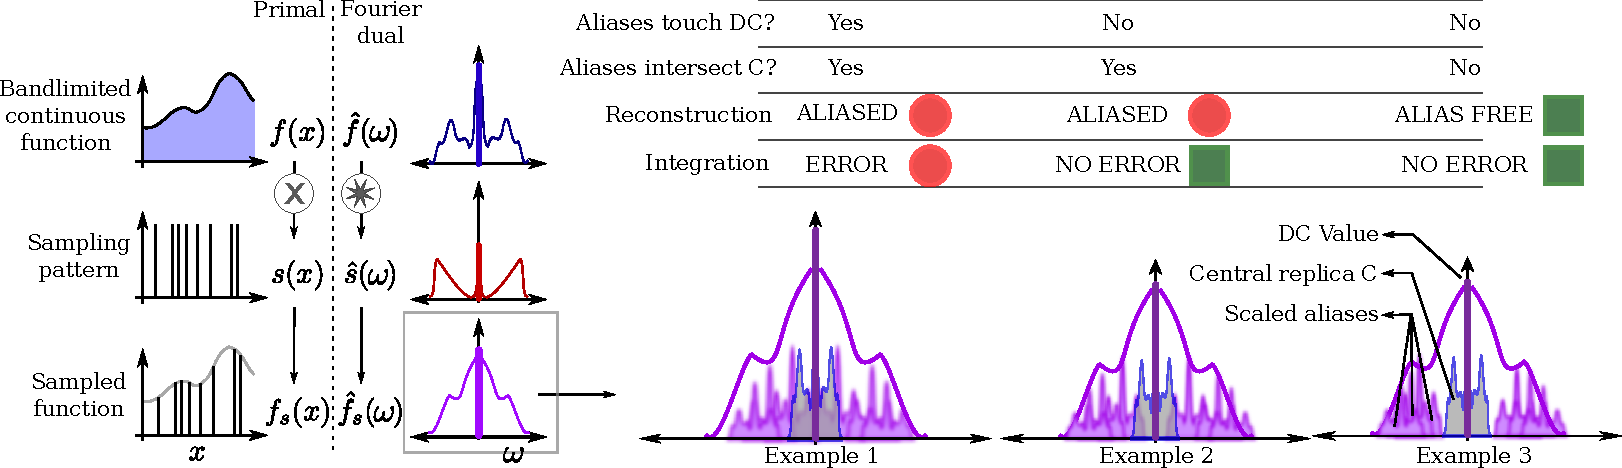
\includegraphics[width=\linewidth]{../CourseNotes/Pictures/IntegRecons.pdf}
%   \caption{Ferrari LaFerrari. Image courtesy Flickr user ``gfreeman23.''}
%   \label{fig:ferrari}
% \end{figure*}

%!TEX root=main.tex
%
% Syllabus and Schedule
%

\definecolor{LightCyan}{rgb}{0.88,0.8,1}
\definecolor{LightBlue}{rgb}{0.75,0.93,1}
\definecolor{LightPink1}{rgb}{1,0.71,0.75}
\definecolor{LightPink2}{rgb}{1,0.75,0.79}	
\definecolor{Mint}{rgb}{0.74,0.98,0.79}
\definecolor{Wheat}{rgb}{0.96,0.87,0.7}

\begin{center}
    \begin{tabular}{ | l | p{5cm} | p{2cm} | p{1.2cm} |}
    \hline
%    \multicolumn{1} { |c| }{Sections} & \multicolumn{1} { c| } {Speakers} & \multicolumn{1} { c| } {Timings} \\
     Sections & Description & Speaker & Duration  \\
    \hline
   \rowcolor{LightCyan}
    & Introduction &  Subr   & 15 \\ 
    \hline
    \rowcolor{Mint} & Probability and Fourier overview  & & \\
    \rowcolor{Mint} & Monte Carlo Integration &  Subr &  20  \\
    \rowcolor{Mint} \multirow{-3}{5cm}{Mathematical Preliminaries} &Sampling and Reconstruction  &  &   \\
    \hline 
    \multicolumn{4} { |c| }{Break (5 mins)} \\ \cline{1-4}
    \hline
     \rowcolor{LightPink1} & Assessing sampling patterns  &  &  \\
     \rowcolor{LightPink1} & Beyond canonical domain & Singh & 15 \\
     \rowcolor{LightPink1} \multirow{-3}{5cm}{Error and sampling analysis} & Manifestation of error & &  \\
    \hline
    \rowcolor{LightBlue} & Classical \& QMC samplers & &   \\
    \rowcolor{LightBlue} & Blue noise samplers & Jarosz   & 15  \\
     \rowcolor{LightBlue} \multirow{-3}{5cm}{Popular samplers} & Synthesising samplers &   &   \\
    \hline
    \rowcolor{Wheat}
    & Case Studies & Jarosz & 10   \\
    \rowcolor{Wheat} \multirow{-3}{5cm}{Experimentation} & Rendering test suite & Subr  & 10  \\
    \hline
    \multicolumn{4} { |c| }{Total (Out of 1.5 hours) = 65 mins (Theory) + 20 mins (Practice) + 5 min (Break) = 90 mins}  \\ \cline{1-4}
    \end{tabular}
\end{center}







% \section*{Acknowledgement}
% Kartic Subr would like to acknowledge funding and encouragement from Royal Society's University Research Fellowship towards this form of scientific dissemination.

\bibliographystyle{acmsiggraph}
% \nocite{*}
\bibliography{2abs}
\end{document}
